\chapter{ \MakeUppercase{El Detector MuTe}}
El telescopio de muones (MuTe) es un detector creado para realizar muografía de volcanes en Colombia. Tiene como característica principal separar los mounes que ingresan al detector de las fuentes de ruido que afectan la muografía. Aplica dos técnicas para el reconocimiento de partículas: la medición del ToF de partículas incidentes y la pérdida de energía.
MuTe esta compuesto por dos detectores: un hodoscopio y un detector Cherenkov de agua (WCD).\\

\begin{figure}[h!]
\begin{center}
\caption{Vista lateral del detector. El WCD contiene 1.7$m^3$ de agua y se ubica sobre el soporte de elevación. El hodoscopio compuesto por dos paneles centelladores de
120 cm × 120 cm ubicados dentro de cajas metálicas que los protegen de la contaminación lumínica y de la humedad.}
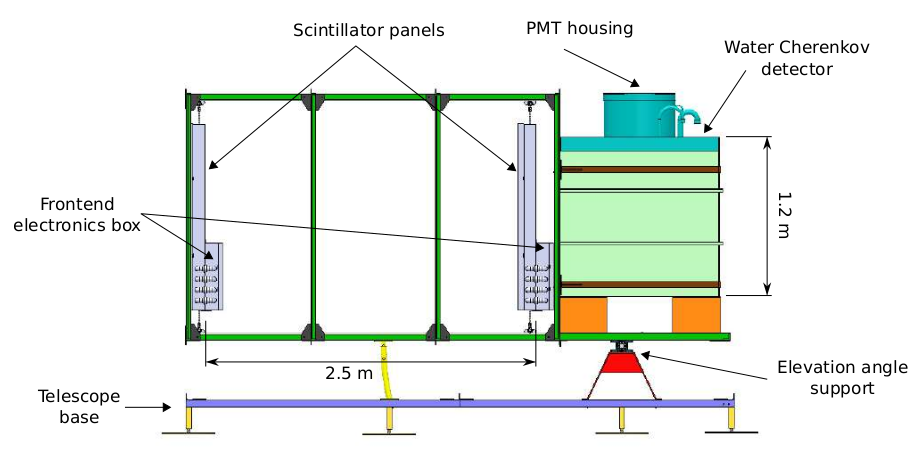
\includegraphics[width=1 \textwidth]{Figures/imagenes/26.png}
\caption*{\textbf{Fuente.} \cite{jesusP}. }
\label{detectores}
\end{center}
\end{figure}


El hodoscopio está conformado por dos paneles sensibles, cada panel contiene 30 barras centelladoras verticales y 30 horizontales, creando una matriz de 900 píxeles. El hodoscopio de MuTe es un dispositivo de conteo de sucesos y su principal función es la estimación del flujo de muones.\\

El WCD es un tanque de acero que contiene 1,7 $m^3$ agua y un tubo fotomultiplicador como elemento sensible. Este detector mide la energía recibida por las partículas cargadas y permite diferenciar los eventos registrados en: muones, electrones/positrones y múltiple partícula.\\

El Sistema ToF de MuTe permite estimar el tiempo que tardan las partículas en atravesar el hodoscopio en una distancia dada y la dirección de estas. Este permite filtrar las partículas que ingresan por la parte posterior. Con el ToF y la energía depositada en el WCD MuTe estima el momentum de las partículas incidentes.

\section{Flujo de datos}

Los datos adquiridos por MuTe son sincronizados temporalmente por un GPS y guardados en dos discos duros, uno para los datos del hodoscopio y otro para los datos del WCD. Cada hora se crean nuevos archivos que almacenan 1 hora de datos. Los datos almacenados tiene meta-datos de presión atmosférica, temperatura y el consumo energético para hacer correcciones de flujo y evaluar la autonomía del detector. Cabe resaltar que estimación del momentum se hace offline.\footcite{jesusP}.
